\section{Process Architecture} \label{ProcessArchitecture}
In this section two distribution diagrams will be shown which explains the processes, the active objects and their connections. All the systems components are on a single process, but there are going to be multiple processes which are communicating with the database. This is due to the system being designed to run on a single process that is not dependent on other process.

\subsection{Distribution Diagrams}
There have been made distribution diagrams, for two of the more complex processes.
The distribution diagram shown in \cref{SLD} will be for the Shopping List.

\begin{figure}[H]
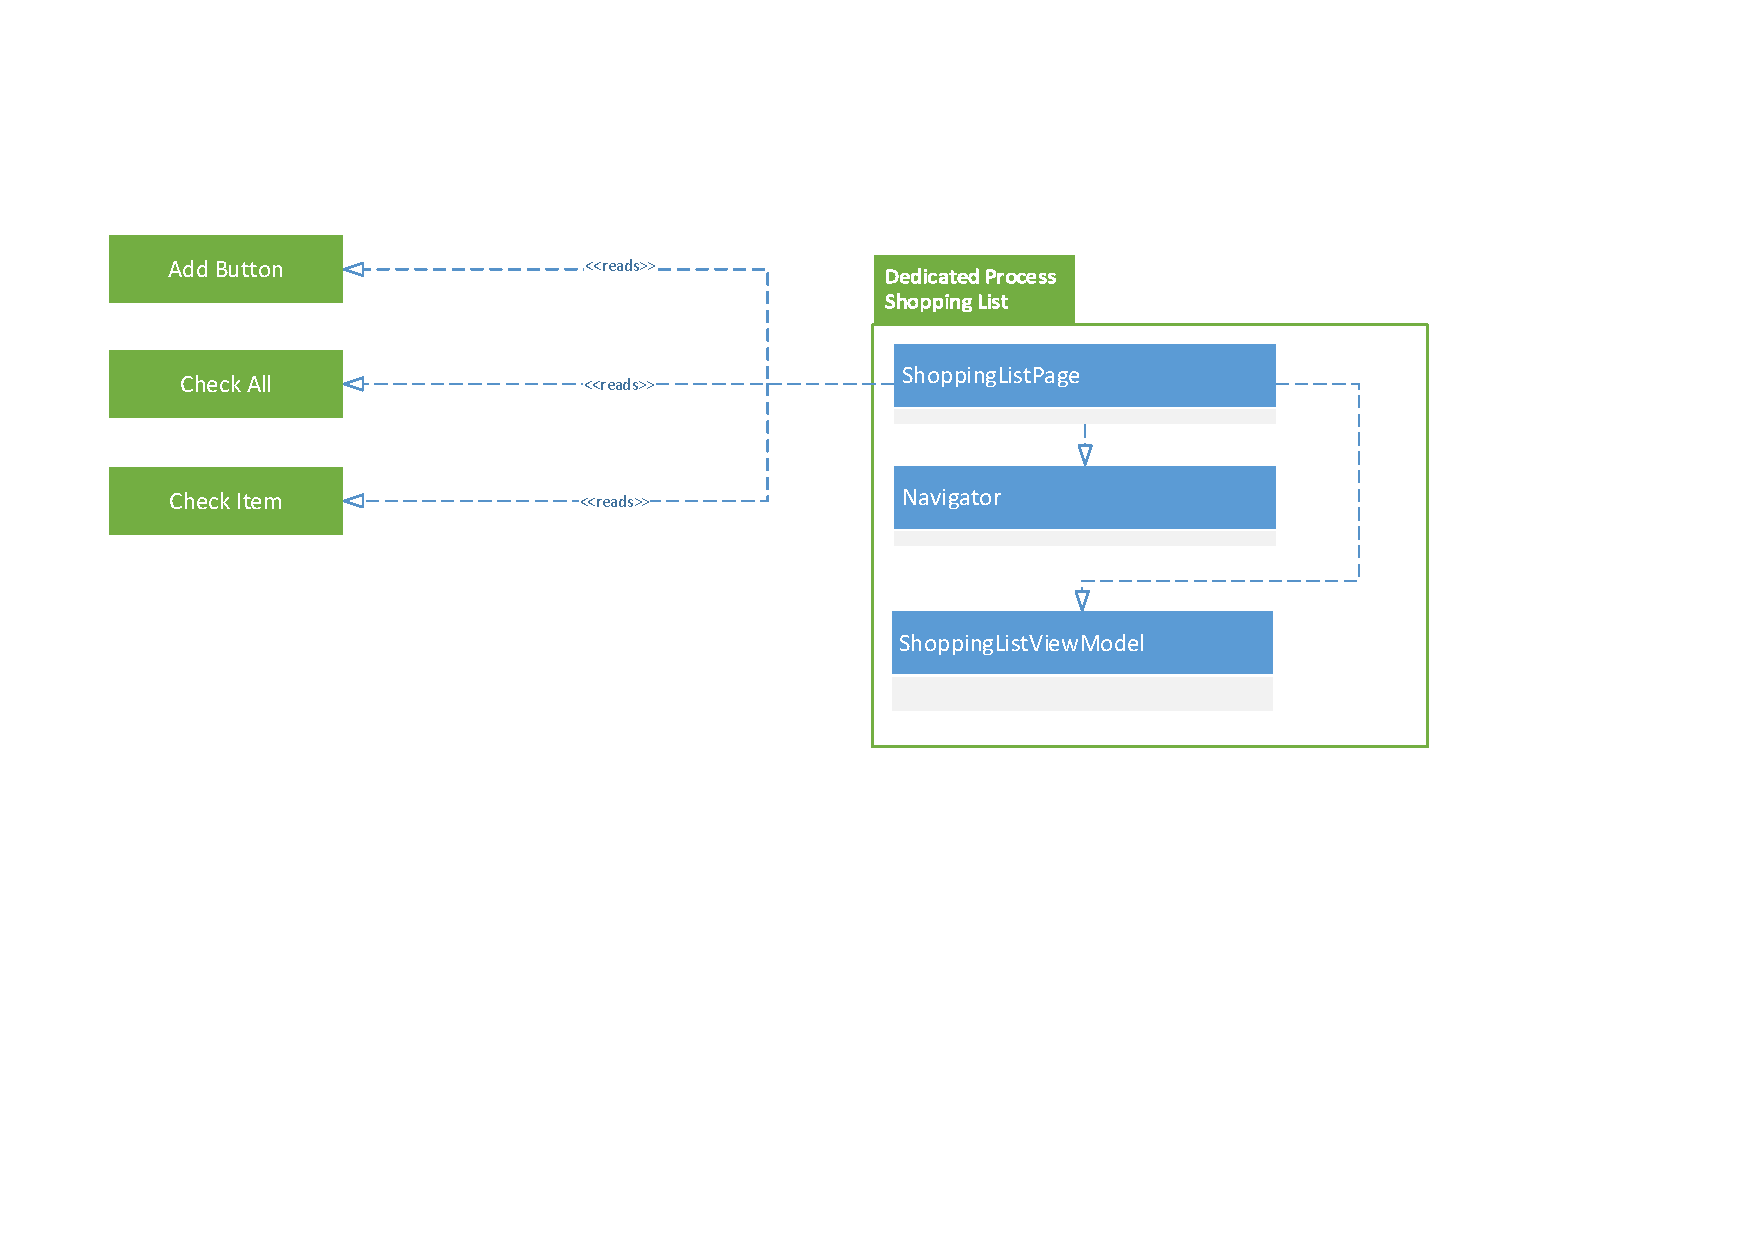
\includegraphics[width =\linewidth, clip=true, trim=1.5cm 8cm 5.5cm 3cm]{Grafik/FoodPlanner/DistributionShoppingList}
\centering
\caption{The distribution diagram for the Shopping List}
\label{SLD}
\end{figure}

\Cref{SLD} shows three active objects:
\begin{itemize}
\item \textbf{Add Button:} This object will add the checked items on the shopping list to the inventory
\item \textbf{Check All:} Checks all items on the shopping list 
\item \textbf{Check Item:} Checks a single item on the shopping list
\end{itemize}

\begin{figure}[H]
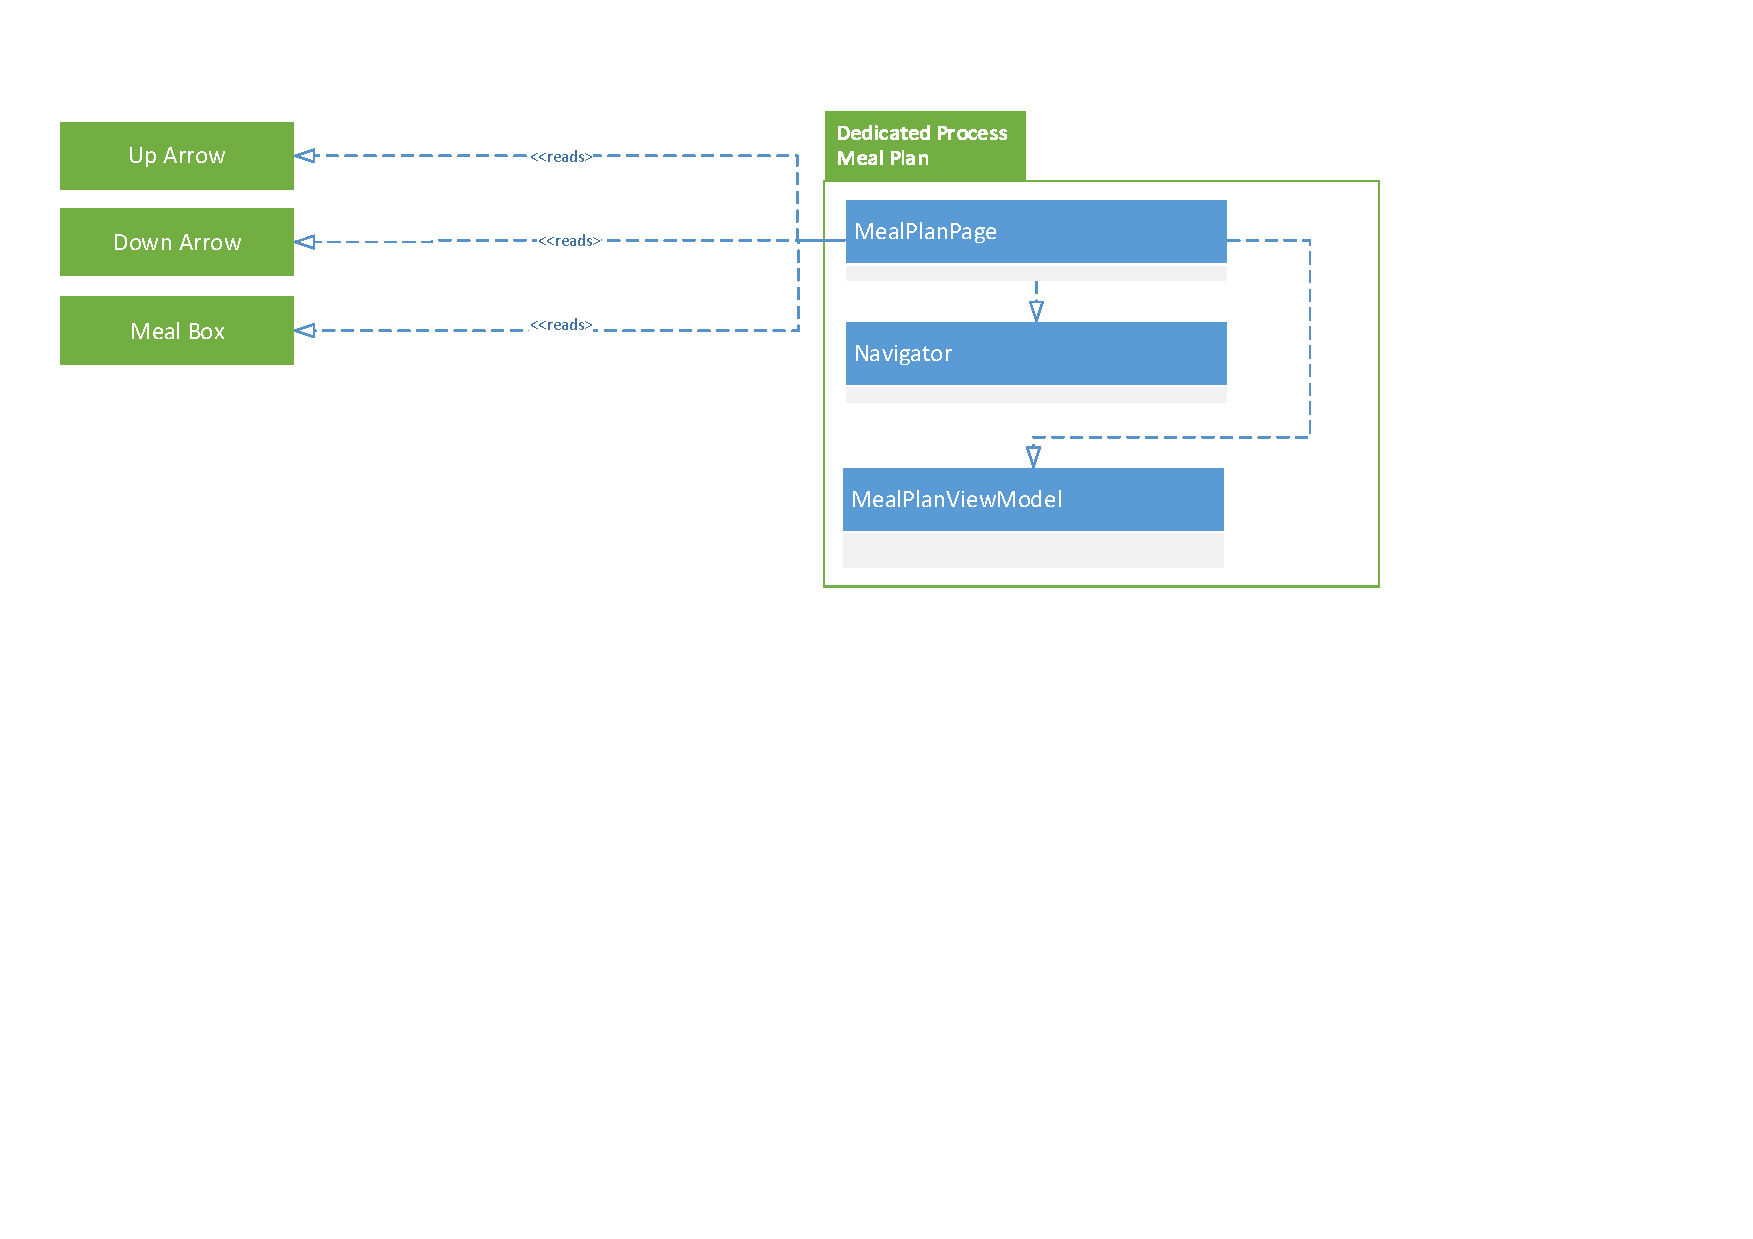
\includegraphics[width=\linewidth, clip=true, trim=0.5cm 10cm 6cm 1.5cm]{Grafik/FoodPlanner/DistributionMealPlan}
\centering
\caption{The distribution diagram for the Meal Plan}
\label{MPD}
\end{figure}

\Cref{MPD} shows three active objects:
\begin{itemize}
\item Up Arrow 
- Displays the previous week
\item Down Arrow 
- Displays the next week
\item Meal Box 
- Sends the user to the Recipe Page
\end{itemize}

The next diagram shows the distribution pattern that will be used.

\begin{figure}[H]
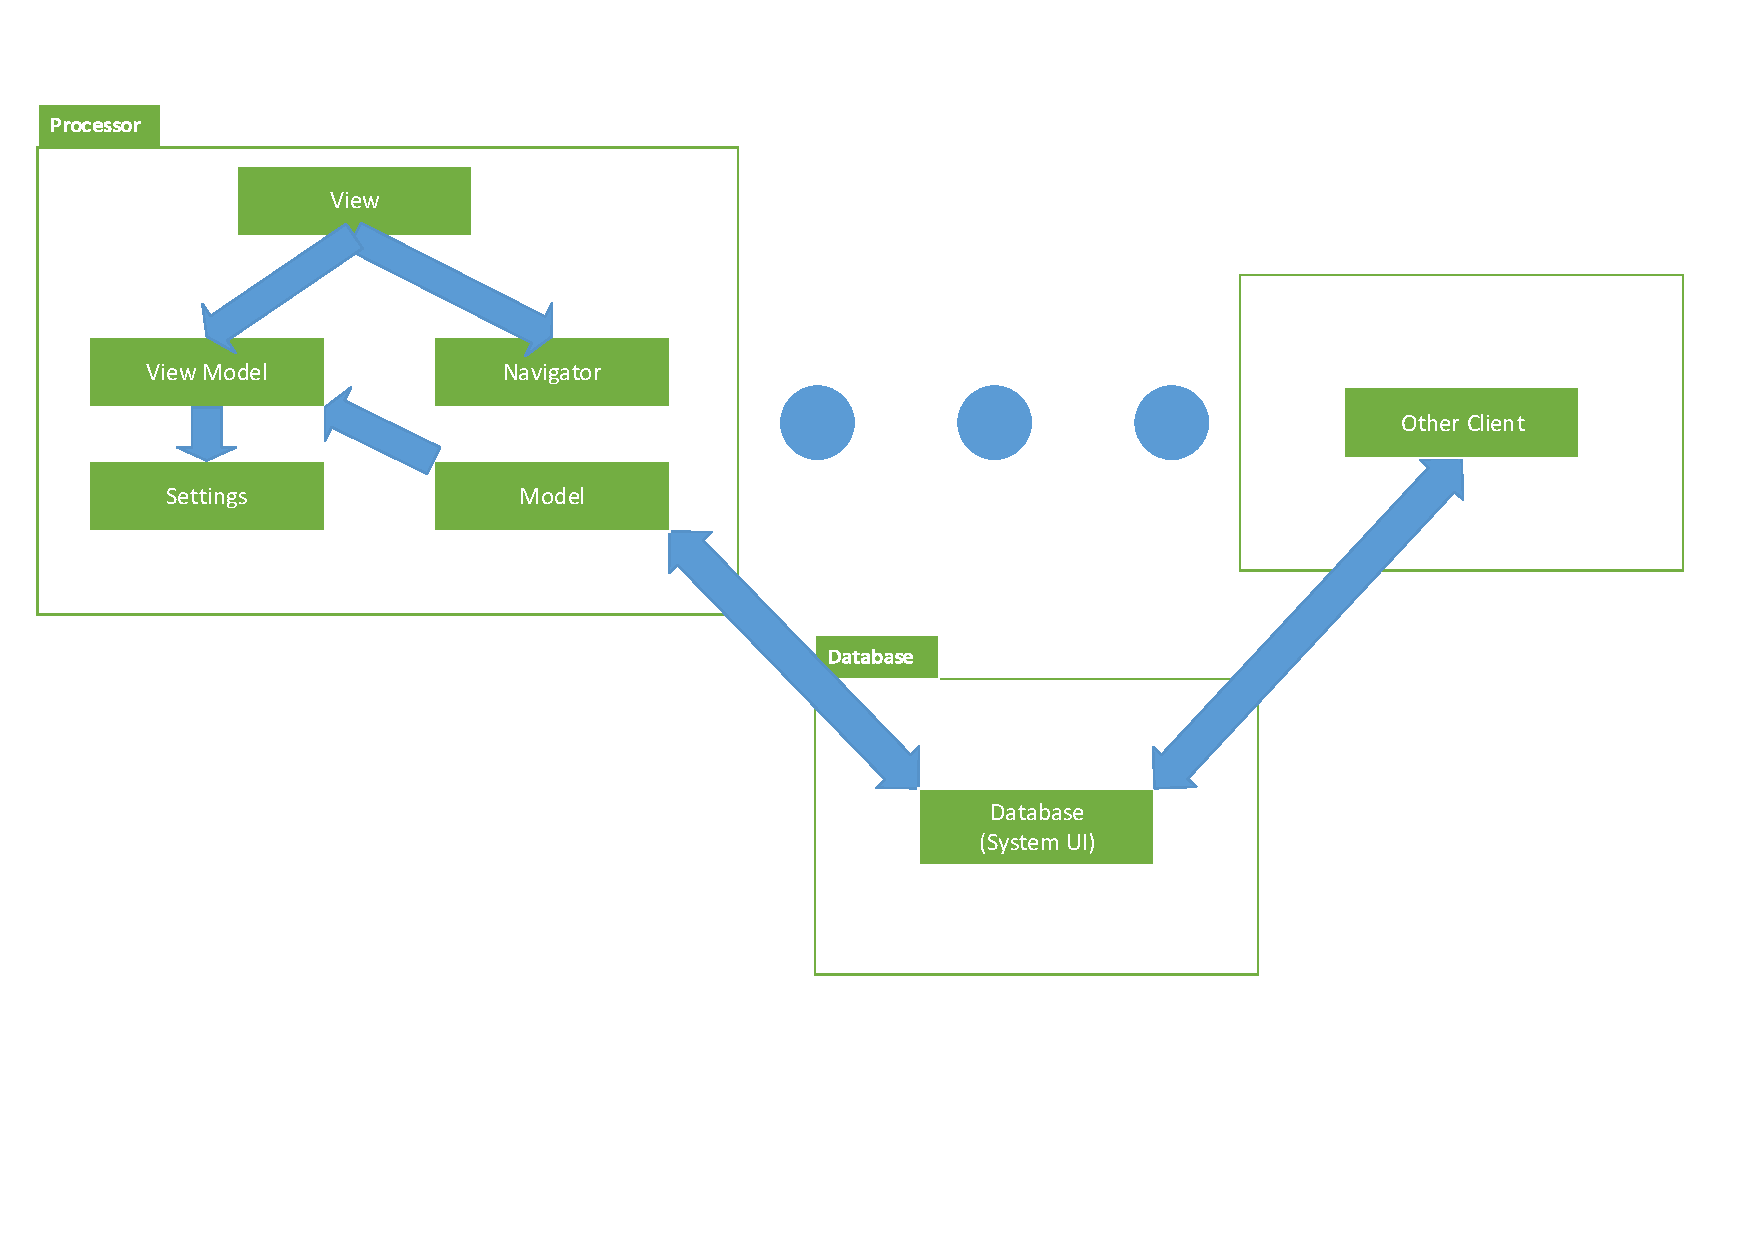
\includegraphics[width=\linewidth, clip=true, trim=0cm 4cm 0.5cm 1cm]{Grafik/FoodPlanner/FordelingsDiagram}
\centering
\caption{The used distribution pattern}
\label{DP}
\end{figure}

\Cref{DP} shows the distribution pattern that will be used, which is a similar pattern to the centralized pattern. Normally the server will perform the functions and keep the model on itself whereas in this system, the client will perform all the functions and still have some local data which is the settings. A downside to this model lies in the stability, as the system is only functional when a clear connection to the server is established. Another downside to the model is the connection time as almost every interaction with the system will require it to communicate with the server. The server communication creates a natural bottleneck in the system as a server can only handle so much data at any time. When the user searches for a recipe, the entire list of recipes will be looked through in order to acquire the matching results. If it was possible to cash data such as recipes or ingredients, data that does not change often, it would loosen the bottleneck.